\chapter{Optical Reference Retrieval with TF-VPR}

\section{Introduction}
Coordinate-missing optical images are difficult to use directly in a multimodal trajectory system. Images with geographic coordinates can be associated with trajectories through their spatial and temporal metadata, while coordinate-missing images only provide visual observations and pixel-level target information. Before these observations can participate in multimodal fusion, the system must first identify visually related coordinate-known references and use them as scene-level anchors.

Visual place recognition provides a natural technical route for this problem. However, as emphasized in the TF-VPR work \cite{wang2026tfvpr}, most strong VPR systems are built around training-intensive pipelines. Single-stage methods learn compact global descriptors for nearest-neighbor retrieval, and two-stage methods combine coarse global retrieval with local feature matching or geometric verification. Although these paradigms are effective, they usually require annotated place pairs, task-specific loss design, hard-negative mining, and large-scale optimization. Such assumptions are not suitable for the coordinate-missing optical setting considered in this thesis, where new scenes may lack reliable place labels and additional VPR training data.

Recent vision foundation models provide a different opportunity. Models such as CLIP, ViT, MAE, and DINOv2 contain transferable visual representations learned from large-scale pretraining. Instead of fine-tuning these models for every new scene, TF-VPR investigates a training-free paradigm in which descriptors are generated, refined, and matched only at test time. This paradigm reduces dependence on annotated datasets, avoids scene-specific optimization, and enables direct reuse of frozen visual features.

Following this idea, this chapter uses TF-VPR as the optical reference retrieval module in the proposed trajectory completion framework. The module retrieves coordinate-known reference images for each coordinate-missing optical image. These retrieved references do not directly produce an absolute geographic trajectory; rather, they provide a constrained candidate set for the downstream target association model. The target association model then links pixel-level target observations to existing target or trajectory identifiers.

Therefore, the contribution of this chapter is not to propose a new target-level matching network, but to organize a training-free optical reference retrieval process that bridges coordinate-missing optical observations and the multimodal fusion pipeline. The following sections define the retrieval problem, describe the TF-VPR-based descriptor generation and Top-\(k\) retrieval process, and explain how the retrieved references are integrated with downstream target association.

\section{Related Work}
This section extends the brief overview of visual place recognition in Chapter 1 and focuses on the literature most relevant to the optical reference retrieval module. The discussion is organized around four lines of work: conventional VPR, graph-based VPR, VFM-based VPR, and training-free visual adaptation.

\subsection{Visual Place Recognition}
Visual place recognition (VPR) determines whether a query image depicts a previously observed place. It is a core component of robotic localization, loop-closure detection, long-term navigation, and large-scale visual retrieval \cite{yin2025gprs,murartal2017orbslam2,milford2008seqslam}. Unlike generic image retrieval, VPR must remain reliable under viewpoint changes, illumination variation, seasonal shifts, occlusion, dynamic objects, and domain shift. These factors are also present in the optical images studied in this thesis, especially when images are collected under different observation conditions or lack reliable geographic coordinates.

Early VPR methods relied mainly on hand-crafted local features and aggregation strategies, including Bag-of-Words and VLAD \cite{galvez2012bags,jegou2010vlad}. These methods are computationally efficient and easy to deploy, but their representation capacity is limited under large appearance changes. With the development of deep learning, CNN-based and Transformer-based methods have become the dominant approach. Existing VPR pipelines can be broadly divided into single-stage and two-stage paradigms \cite{wang2026tfvpr}.

As shown in Fig.~\ref{fig:tfvpr-single-stage-vpr}, single-stage methods encode each image into a compact global descriptor and retrieve reference images through nearest-neighbor search. NetVLAD introduced a learnable VLAD-style aggregation layer for weakly supervised place recognition \cite{arandjelovic2016netvlad}. Patch-NetVLAD further improved retrieval by combining local and global descriptors at multiple scales \cite{hausler2021patchnetvlad}. More recent methods, including CosPlace, EigenPlaces, and MixVPR, improve descriptor discriminability through better training data construction, viewpoint-robust learning, and feature mixing \cite{berton2022cosplace,berton2023eigenplaces,alibey2023mixvpr}.

Two-stage VPR pipelines use a coarse-to-fine retrieval process. As illustrated in Fig.~\ref{fig:tfvpr-two-stage-vpr}, a global descriptor first retrieves candidate reference images, and local feature matching or geometric verification then reranks these candidates. This design can improve robustness under viewpoint and structural changes by combining global scene-level cues with local spatial correspondences. However, both single-stage and two-stage learning-based paradigms often rely on annotated training data, task-specific losses, and hard-negative mining. These requirements are restrictive in newly observed scenes where coordinate labels, place correspondences, or retrieval annotations are unavailable. For the coordinate-missing optical setting in this thesis, the retrieval module must therefore operate without additional scene-specific VPR training.

\begin{figure}[!htbp]
  \centering
  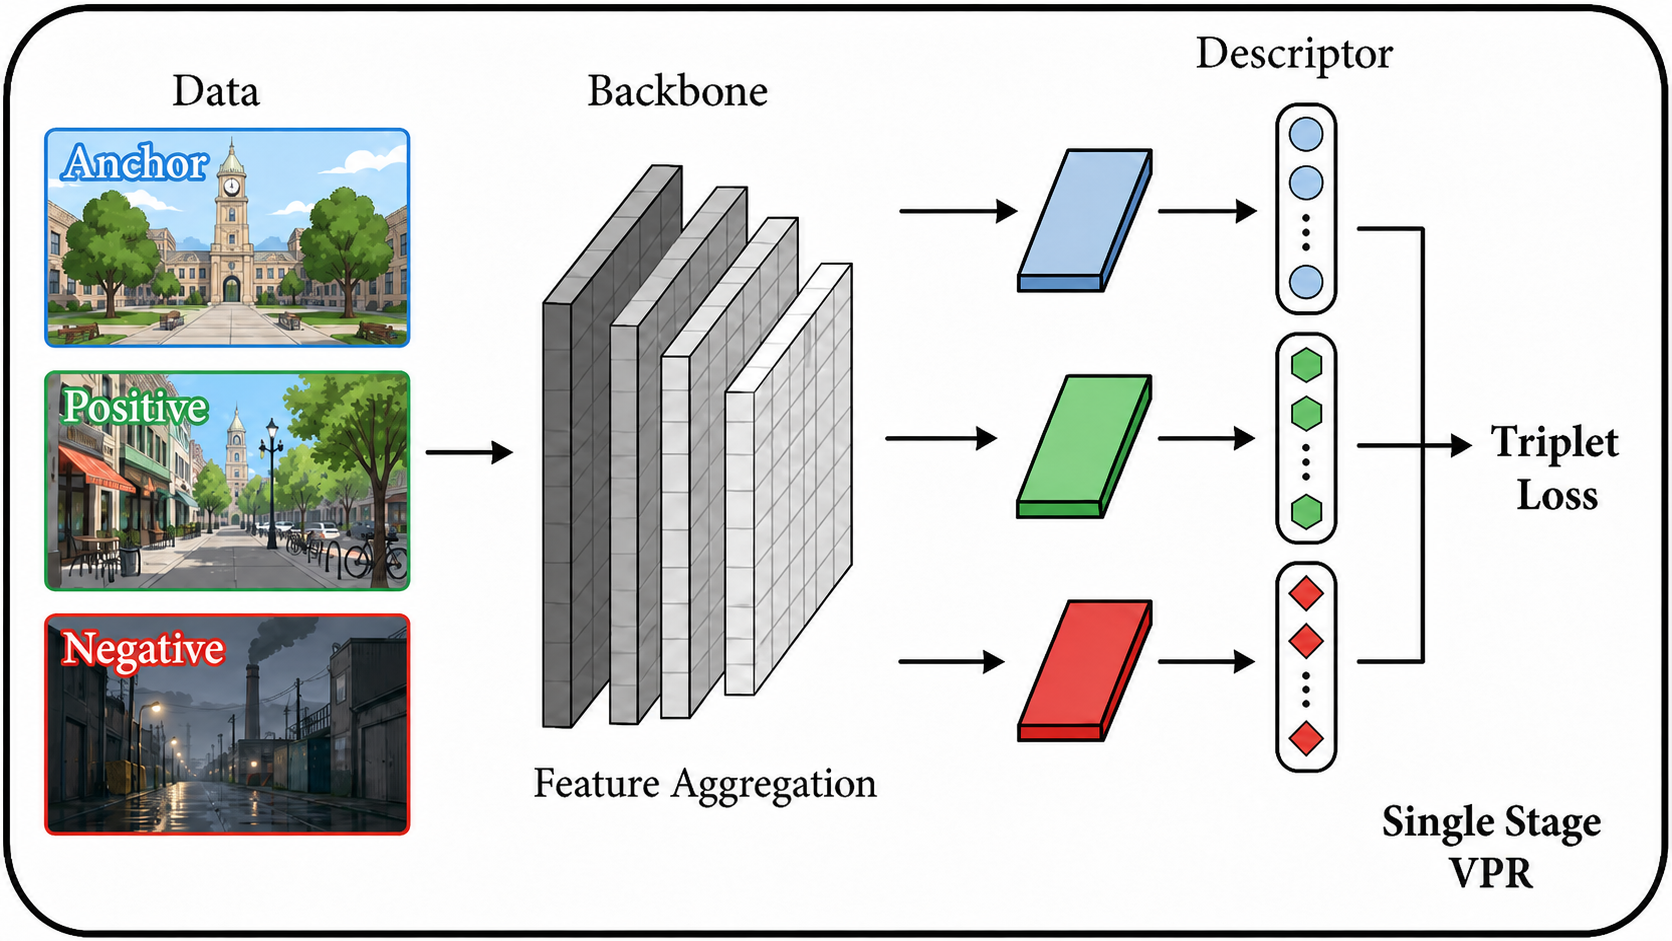
\includegraphics[width=0.88\linewidth,height=0.28\textheight,keepaspectratio]{images/chapter3/single_stage_vpr_pipeline.png}
  \caption{Single-stage VPR pipeline. A query image is encoded by a backbone into a compact global descriptor, and reference images are retrieved by nearest-neighbor search \cite{arandjelovic2016netvlad,hausler2021patchnetvlad}.}
  \label{fig:tfvpr-single-stage-vpr}
\end{figure}

\begin{figure}[!htbp]
  \centering
  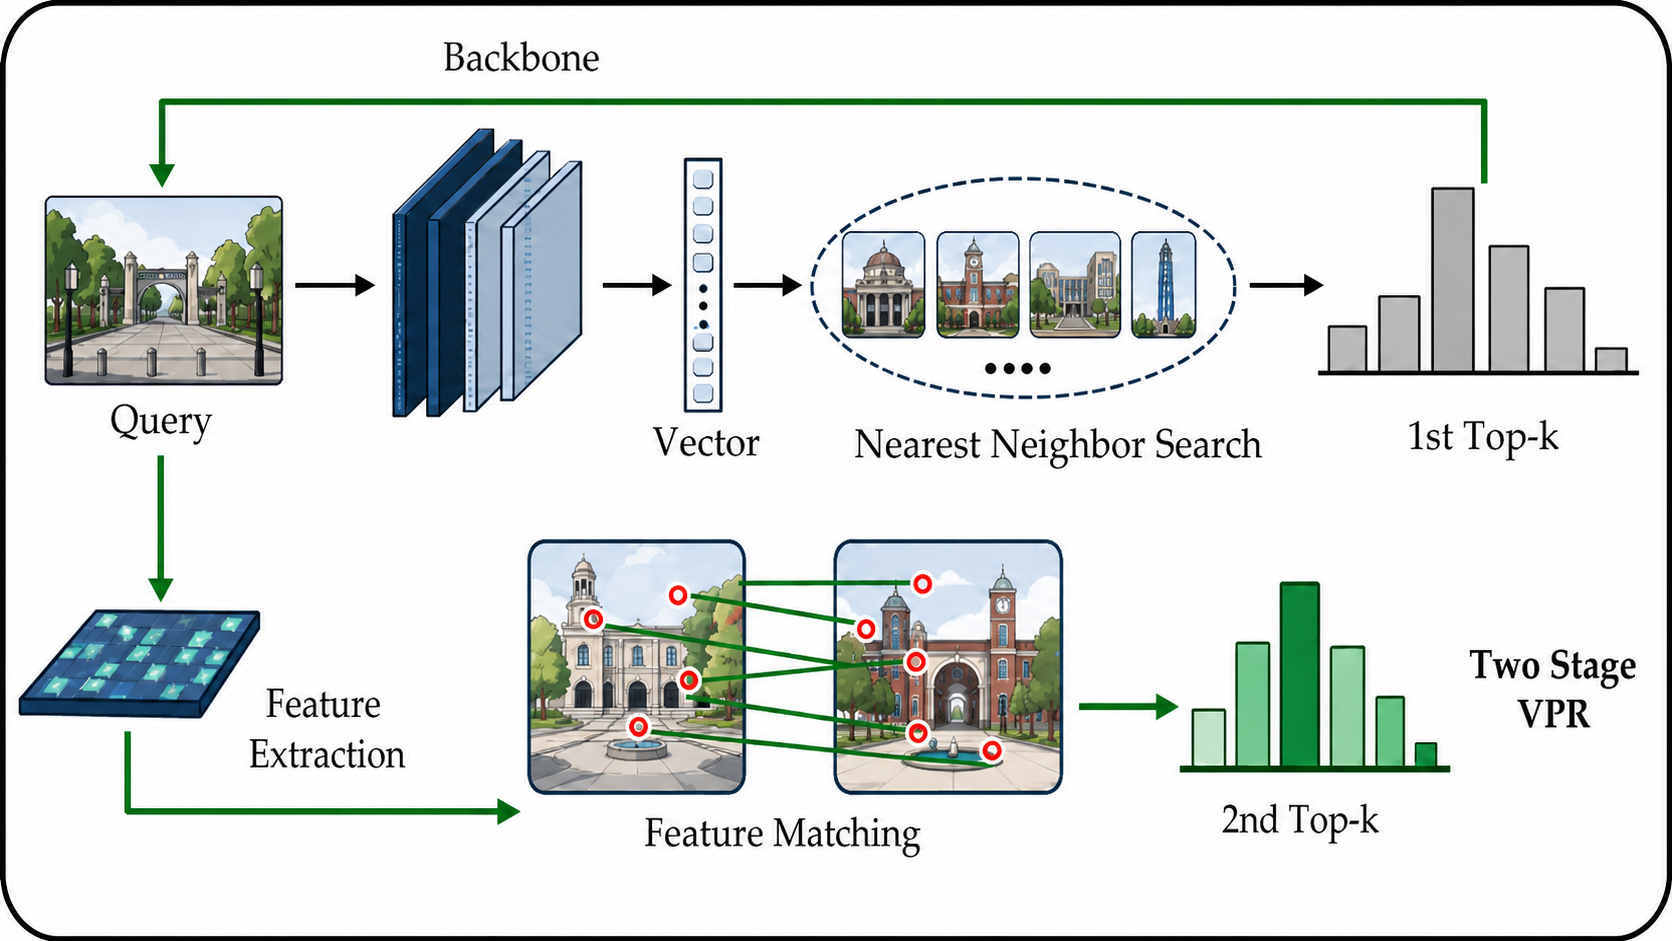
\includegraphics[width=0.88\linewidth,height=0.28\textheight,keepaspectratio]{images/chapter3/two_stage_vpr_pipeline.png}
  \caption{Two-stage VPR pipeline. A global descriptor first retrieves candidate references, and local feature matching then reranks the candidates to obtain a refined Top-k result for more reliable place recognition.}
  \label{fig:tfvpr-two-stage-vpr}
\end{figure}

\subsection{Graph-Based Visual Place Recognition}
Graph-based VPR methods improve retrieval robustness by modeling spatial or semantic relationships among image regions. Rather than treating an image descriptor as a single pooled vector, these methods represent patches, regions, or semantic components as graph nodes and use their relationships for place matching. Qin et al. use learnable feature-map filtering and graph attention networks to model dependencies among feature regions \cite{qin2021gatvpr}. PRGS introduces patch-to-region graph search to improve robustness under viewpoint variation \cite{zuo2025prgs}. SAGE further combines spatial-visual graph exploration with parameter-efficient fine-tuning and dynamic hard-sample mining \cite{chen2025sage}.

These studies show that graph reasoning is useful for VPR because stable spatial structures are often more reliable than isolated visual responses. However, most graph-based VPR methods still require task-specific training or fine-tuning. This limits their direct applicability to coordinate-missing optical images, where labeled VPR pairs may not exist. The TF-VPR strategy adopted in this chapter retains the structural motivation of graph-based VPR while avoiding learned graph parameters. Its Training-Free Graph-Attention Module constructs token relationships directly from frozen visual features and performs parameter-free feature refinement. This makes graph reasoning more suitable for deployment without scene-specific annotation.

\subsection{VFM-Based Visual Place Recognition}
Vision foundation models (VFMs), including CLIP, ViT, MAE, and DINOv2, have shown strong general visual representation ability through large-scale pretraining \cite{radford2021clip,dosovitskiy2020vit,he2022mae,oquab2023dinov2}. Their emergence creates a practical opportunity for VPR. Instead of training a place recognition model from scratch, one can reuse frozen visual representations and evaluate how well they support place retrieval. AnyLoc is a representative training-free VFM-based VPR method. It applies off-the-shelf DINOv2 features with pooling strategies such as GeM or VLAD \cite{keetha2024anyloc}. Its results indicate that frozen VFM features can provide strong zero-shot place recognition across diverse environments.

Simple pooling over frozen VFM tokens, however, may not fully exploit spatial structure or cross-image alignment. In contrast, SALAD introduces an optimal-transport-based aggregation strategy and a dustbin cluster to suppress distractors, including sky regions and dynamic objects, but it requires training or fine-tuning \cite{izquierdo2024salad}. This contrast defines a methodological gap. Training-free VFM features are flexible and annotation-efficient, whereas trained aggregation modules often produce stronger descriptors but reduce deployment flexibility. TF-VPR is positioned in this gap. It keeps the backbone frozen, as in training-free VFM-based methods, and introduces deterministic attention-based refinement to improve descriptor discriminability without additional training \cite{wang2026tfvpr}.

\subsection{Training-Free Visual Adaptation}
Training-free methods in related visual tasks provide useful inspiration for TF-VPR. In training-free segmentation and open-vocabulary dense prediction, frozen foundation models are adapted at inference time by manipulating token interactions, attention maps, or prototype representations rather than updating model parameters. Methods such as MaskCLIP and CLIP-based dense prediction show that frozen vision-language or visual backbones already encode useful dense semantics, although their raw attention responses may contain noise or spatial inconsistency \cite{ding2023maskclip,sun2024clipasrnn}. These observations suggest that performance can often be improved by refining how frozen features are read and aggregated, even when model weights remain unchanged.

Zero-shot classification methods provide another related perspective. Parameter-free attention, non-parametric memory, and test-time calibration strategies can improve the use of frozen features without supervised fine-tuning \cite{guo2023calip,zanella2024testtime}. These ideas are compatible with the deployment requirement of this thesis. The system should process coordinate-missing optical images from new scenes without constructing an additional labeled training set. Therefore, the focus shifts from learning new parameters to extracting, refining, and comparing frozen visual features in a deterministic and reproducible way.

Based on this literature, this chapter adopts TF-VPR as the optical reference retrieval module. As summarized in Fig.~\ref{fig:tfvpr-training-free-benchmark}, its key difference from training-based VPR is that descriptor generation uses a frozen backbone and deterministic aggregation at test time. It does not optimize the backbone or aggregation module on a dedicated VPR training set. The module uses frozen VFM representations and training-free attention mechanisms to retrieve coordinate-known reference images for coordinate-missing optical images. These retrieved references then constrain downstream target association, which links pixel-level observations to target or trajectory identifiers. In this chapter, TF-VPR is used primarily as a scene-level candidate retrieval stage, while target-level correspondence is handled by the downstream association module. In this way, TF-VPR provides the retrieval bridge between coordinate-missing optical images and the multimodal target fusion module developed in the next chapter.

\begin{figure}[!htbp]
  \centering
  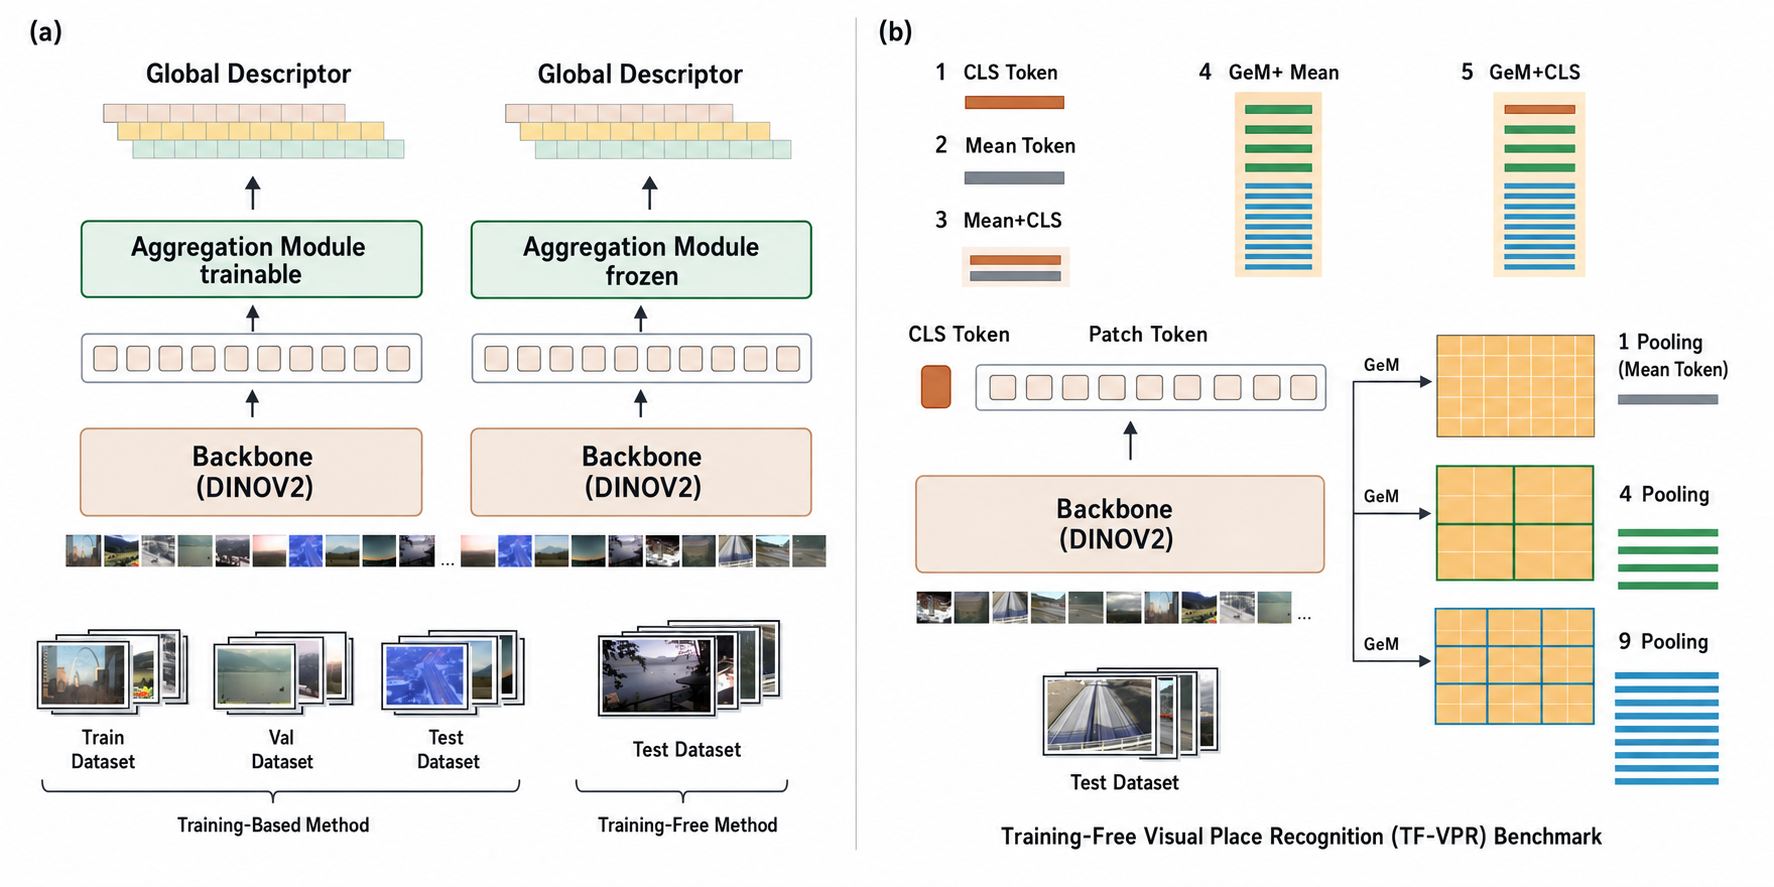
\includegraphics[width=\linewidth,height=0.38\textheight,keepaspectratio]{images/chapter3/tf_vpr_overview.png}
  \caption{Training-free VPR motivation and descriptor benchmark. TF-VPR differs from training-based VPR by keeping the DINOv2 backbone and aggregation process fixed during deployment, and it compares several frozen-token aggregation choices such as CLS, mean, and GeM-based descriptors \cite{wang2026tfvpr}.}
  \label{fig:tfvpr-training-free-benchmark}
\end{figure}

\section{Problem Definition}
Let \(I_u\) denote a set of coordinate-missing optical images, and let \(I_r\) denote a set of coordinate-known reference optical images. The existing trajectory set is denoted as \(T_r\), which may be obtained from coordinate-known optical images or other sensing modalities. For each image in \(I_u\), pixel-level target observations are denoted as \(O_u\), including target boxes, target centers, or local target patches.

The objective of this chapter is to retrieve reliable reference images from \(I_r\) for each coordinate-missing image in \(I_u\), and then use downstream target association results to connect \(O_u\) to the existing trajectory system. The output of this chapter is not an absolute geographic trajectory recovered directly from pixels. Instead, the output is a trajectory association record or a completed optical trajectory segment that can be used by the multimodal fusion module in the next chapter.

\section{TF-VPR Method}
The TF-VPR module is responsible for image-level candidate reference retrieval. It generates image descriptors from a frozen vision foundation model and refines them using training-free attention mechanisms. Since no additional training or fine-tuning is required, the module is suitable for scenes where labeled VPR training data are unavailable. The overall pipeline is shown in Fig.~\ref{fig:tfvpr-method-framework}: the frozen backbone first extracts patch tokens, TF-GAM refines them through graph-style propagation, TF-CAM aggregates them with prototype-guided cross-attention, and the resulting global descriptor is used for image-level retrieval.

\begin{figure}[!htbp]
  \centering
  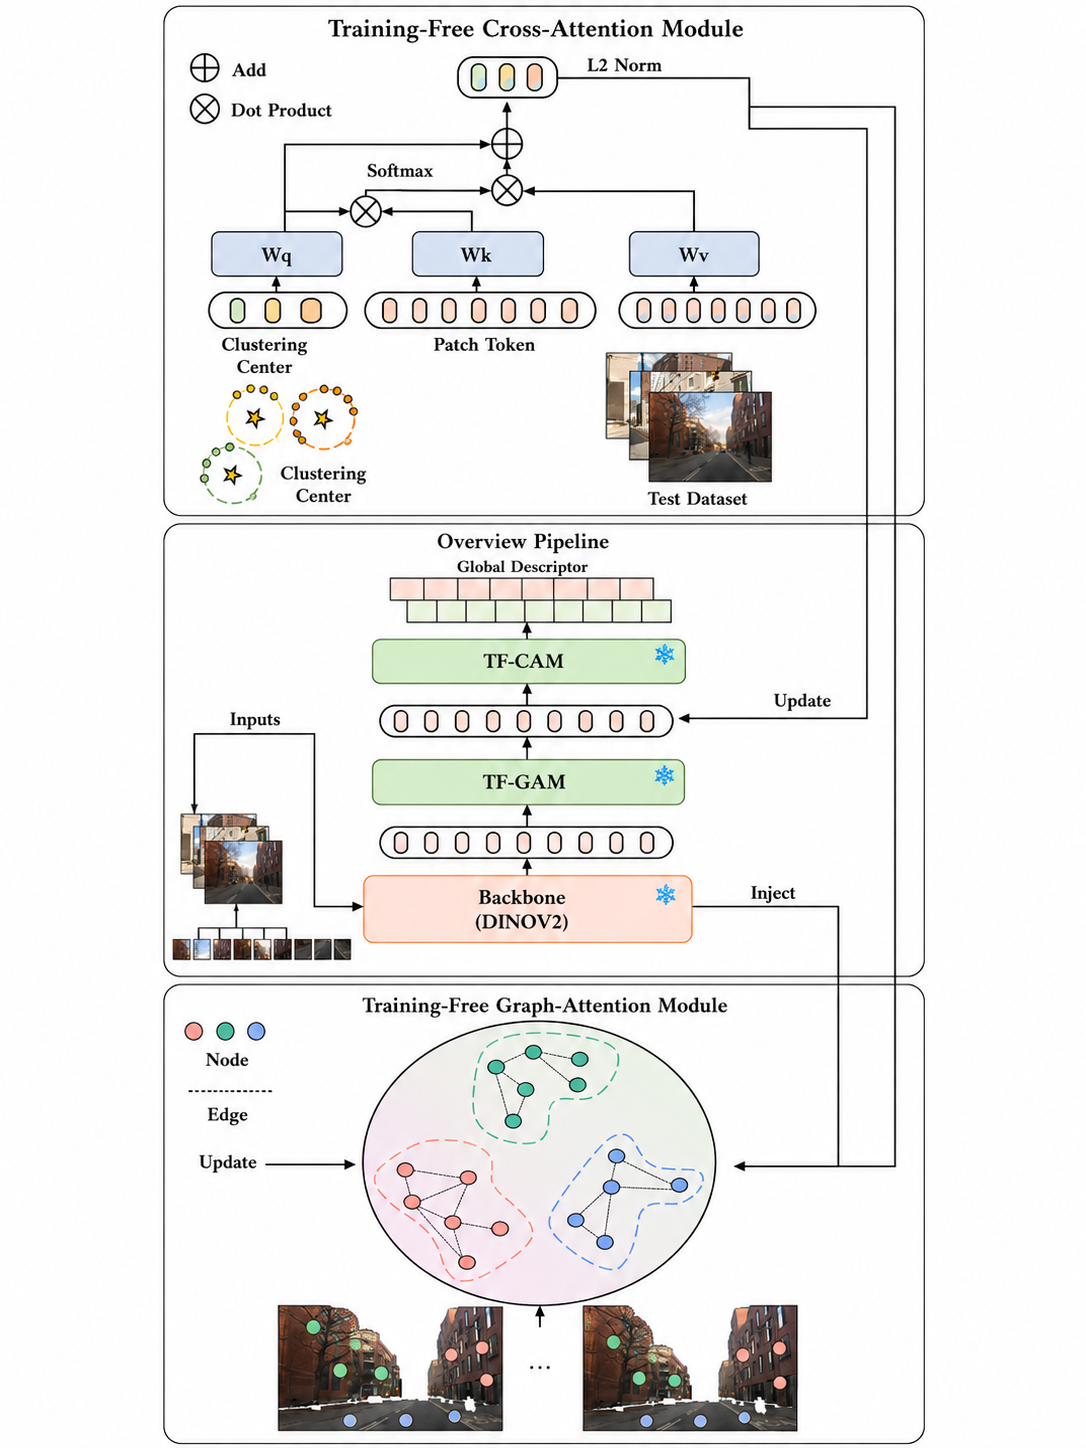
\includegraphics[width=\linewidth,height=0.40\textheight,keepaspectratio]{images/chapter3/tf_vpr_method.png}
  \caption{TF-VPR framework. The method combines frozen DINOv2 feature extraction, a Training-Free Graph-Attention Module, and a Training-Free Cross-Attention Module to generate global descriptors for training-free visual place recognition \cite{wang2026tfvpr}.}
  \label{fig:tfvpr-method-framework}
\end{figure}

\subsection{Training-Free VPR Framework}
Given an input image, a frozen visual encoder extracts a class token and a set of patch tokens. These features are used to build an image descriptor through deterministic operations. Unlike training-based VPR methods, the backbone parameters remain fixed, and all descriptor generation, refinement, and matching operations are performed at inference time.

More specifically, following the TF-VPR formulation \cite{wang2026tfvpr}, let \(f_{\theta}\) denote a pretrained visual foundation model with fixed parameters \(\theta\). For an image \(I\), the backbone outputs a class token \(x_{\mathrm{cls}} \in \mathbb{R}^{d}\) and \(N\) patch tokens:
\begin{equation}
  X = [x_1; x_2; \ldots; x_N] \in \mathbb{R}^{N \times d}.
\end{equation}
The goal of training-free VPR is to construct a global image descriptor \(g(I)\) through a deterministic and label-free mapping:
\begin{equation}
  g(I) = \phi(x_{\mathrm{cls}}, X),
\end{equation}
where \(\phi(\cdot)\) contains no trainable parameters and does not use annotated place pairs, triplets, hard negatives, or scene-specific losses. After descriptor generation, all descriptors are \(L_2\)-normalized and compared by cosine similarity.

Simple training-free baselines can be expressed within the same framework. The class-token baseline directly uses \(g_{\mathrm{CLS}}(I)=\operatorname{Norm}(x_{\mathrm{cls}})\). The mean-token baseline uses the normalized average of all patch tokens:
\begin{equation}
  g_{\mathrm{Mean}}(I) =
  \operatorname{Norm}\left(\frac{1}{N}\sum_{i=1}^{N}x_i\right).
\end{equation}
Other variants concatenate the class token with pooled patch descriptors, or apply GeM pooling over multiple spatial grids before normalization. These baselines are simple and reproducible, but they do not explicitly model local structure or cross-image semantic alignment.

TF-VPR addresses this limitation with a cascaded training-free pipeline. First, TF-GAM refines patch tokens within each image by propagating information along a sparse token-similarity graph. Second, TF-CAM aggregates the refined tokens by using unsupervised clustering centers as fixed queries, which projects images into a shared prototype-based descriptor space. In the coordinate-missing optical setting of this thesis, this design is useful because the system must retrieve coordinate-known references without collecting new VPR labels for each scene.

This training-free design reduces the dependence on annotated place recognition data and avoids task-specific optimization. In the context of this thesis, this property is important because coordinate-missing optical images may come from new scenes where additional VPR training data are not available.

\subsection{Training-Free Graph-Attention Module}
The Training-Free Graph-Attention Module refines patch-level visual features by modeling local structural relations among image patches. Patch tokens extracted from the frozen visual encoder are treated as nodes, and their similarities are used to construct a graph-like relation structure. Through parameter-free attention-based propagation, local structural consistency can be enhanced without updating model weights.

In conventional graph attention modules, node features are usually transformed by learned query, key, and value projections, and the attention parameters are optimized through gradient descent. TF-GAM removes these learned projections. Given the patch token matrix \(X \in \mathbb{R}^{N \times d}\), it directly sets
\begin{equation}
  Q = K = V = X.
\end{equation}
The pairwise token affinity matrix is then computed from normalized dot-product similarity:
\begin{equation}
  S = \frac{QK^{\top}}{\sqrt{d}} \in \mathbb{R}^{N \times N}.
\end{equation}
For each token \(i\), only the indices of the top-\(k\) most similar tokens are retained as its neighborhood \(\mathcal{N}_{k}(i)\). The masked affinity matrix is defined as
\begin{equation}
  \tilde{S}_{ij} =
  \begin{cases}
    S_{ij}, & j \in \mathcal{N}_{k}(i),\\
    -\infty, & \text{otherwise}.
  \end{cases}
\end{equation}
Applying row-wise softmax gives the sparse attention matrix \(A=\operatorname{Softmax}(\tilde{S})\). The graph-refined patch tokens are obtained by
\begin{equation}
  X_{\mathrm{att}} = AV.
\end{equation}
Finally, TF-GAM uses a residual convex combination to preserve the original token identity while injecting neighborhood context:
\begin{equation}
  X_{\mathrm{GAM}} = \lambda X + (1-\lambda)X_{\mathrm{att}},
\end{equation}
where \(\lambda\) controls the balance between the raw frozen features and the graph-propagated features. In the TF-VPR experiments, sparse neighborhoods and a residual weight around the high-preservation range are shown to be more stable than fully replacing raw features with propagated features \cite{wang2026tfvpr}.

The purpose of this module is to suppress unstable or isolated visual responses and strengthen coherent scene structures. This is useful for place recognition because stable structural regions usually provide more reliable cues than transient or noisy image regions.

This design is particularly relevant to coordinate-missing optical images. When viewpoint, illumination, occlusion, or dynamic targets disturb individual patches, raw patch tokens may produce noisy local responses. The top-\(k\) graph prevents every patch from attending to all other patches and reduces spurious long-range interactions. The residual update then reinforces semantically coherent structures such as roads, facades, and stable background regions while avoiding excessive smoothing. Therefore, TF-GAM provides a training-free way to make the subsequent global descriptor less sensitive to local visual noise.

\subsection{Training-Free Cross-Attention Module}
The Training-Free Cross-Attention Module aggregates graph-refined patch tokens into a compact and more comparable global descriptor. Its main purpose is to address a limitation that remains after TF-GAM. Although TF-GAM improves intra-image structural coherence, descriptors from different images may still be difficult to compare if their patch tokens are pooled without a shared reference frame. TF-CAM therefore introduces unsupervised clustering prototypes as fixed semantic anchors and uses them as queries in a parameter-free cross-attention operation \cite{wang2026tfvpr}.

The prototypes are constructed offline without labels. A pool of patch tokens is first sampled from database images or from another unlabeled image corpus:
\begin{equation}
  \mathcal{S} = \{u_1,u_2,\ldots,u_M\}, \quad u_m \in \mathbb{R}^{d}.
\end{equation}
K-means clustering is then applied to this token pool to obtain \(K\) centroids:
\begin{equation}
  P = [p_1;p_2;\ldots;p_K] \in \mathbb{R}^{K \times d}.
\end{equation}
These centroids are fixed after construction and are not optimized with place labels. In the original TF-VPR implementation, \(K=16\) is used as the default number of clustering centers, which provides a balance between descriptor compactness and prototype expressiveness \cite{wang2026tfvpr}. Since the clustering process only uses unlabeled tokens, it satisfies the training-free constraint of the benchmark.

For an input image, let \(X_{\mathrm{GAM}} \in \mathbb{R}^{N \times d}\) denote the patch tokens refined by TF-GAM. TF-CAM treats the prototype matrix \(P\) as the query matrix, while the graph-refined patch tokens serve as keys and values:
\begin{equation}
  Q_{\mathrm{CAM}} = P, \quad
  K_{\mathrm{CAM}} = X_{\mathrm{GAM}}, \quad
  V_{\mathrm{CAM}} = X_{\mathrm{GAM}}.
\end{equation}
The prototype-to-patch attention score is computed as
\begin{equation}
  S_{\mathrm{CAM}} =
  \frac{Q_{\mathrm{CAM}}K_{\mathrm{CAM}}^{\top}}{\sqrt{d}}
  \in \mathbb{R}^{K \times N}.
\end{equation}
After row-wise softmax, each prototype obtains an attention distribution over all refined patch tokens:
\begin{equation}
  W_{\mathrm{CAM}} = \operatorname{Softmax}(S_{\mathrm{CAM}}).
\end{equation}
The prototype-aligned feature matrix is then obtained by weighted aggregation:
\begin{equation}
  F_{\mathrm{CAM}} = W_{\mathrm{CAM}}V_{\mathrm{CAM}}
  \in \mathbb{R}^{K \times d}.
\end{equation}
Each row of \(F_{\mathrm{CAM}}\) describes how the image responds to one unsupervised prototype. In this way, different images are projected into the same prototype coordinate system before descriptor comparison.

The final TF-CAM descriptor is produced by vectorizing the prototype-aligned feature matrix and applying \(L_2\) normalization:
\begin{equation}
  g_{\mathrm{CAM}}(I) =
  \operatorname{Norm}\left(\operatorname{vec}(F_{\mathrm{CAM}})\right).
\end{equation}
Following the full TF-VPR setting, this local prototype-aware descriptor can be concatenated with the class token to preserve both local structural information and global semantic context:
\begin{equation}
  g_{\mathrm{TF\mbox{-}VPR}}(I) =
  \operatorname{Norm}\left([x_{\mathrm{cls}};\operatorname{vec}(F_{\mathrm{CAM}})]\right).
\end{equation}
When \(K=16\), the prototype-aware part has dimension \(16 \times d\), and the concatenation with the class token gives the \(17 \times d\) descriptor reported in the experimental tables.

This design improves cross-image comparability because the same prototypes are used for every query and database image. Each centroid can be interpreted as a recurrent visual motif in the unlabeled token distribution, such as facade texture, road surface, vegetation, sky, or foreground structures. Cross-attention aligns image patches to these anchors, which reduces the effect of token permutation, partial occlusion, and local appearance variation. For coordinate-missing optical images, this shared prototype space helps retrieve coordinate-known references that are visually and semantically related to the query image.

The computational cost of TF-CAM is also moderate. The offline clustering step depends on the sampled token count \(M\) and the prototype number \(K\), and it can be performed once before inference. During inference, the main cost is computing \(S_{\mathrm{CAM}}\) and \(F_{\mathrm{CAM}}\), which is \(O(KNd)\) per image. This cost is acceptable for moderate \(K\) and \(N\), especially because it avoids any supervised training or fine-tuning.

\subsection{Similarity Computation and Top-k Retrieval}
After descriptors are generated for coordinate-missing query images and coordinate-known reference images, image-level similarity is computed between them. Let \(g(q)\) denote the normalized descriptor of a query image \(q\), and let \(g(r_j)\) denote the normalized descriptor of the \(j\)-th reference image. The similarity score is computed by cosine similarity:
\begin{equation}
  s(q,r_j) = g(q)^{\top}g(r_j).
\end{equation}
Because all descriptors are \(L_2\)-normalized, this dot product directly measures descriptor similarity.

For each coordinate-missing image, all coordinate-known reference images are ranked by \(s(q,r_j)\). The TF-VPR module outputs the top-\(k\) most similar reference images and their similarity scores:
\begin{equation}
  \mathcal{R}_k(q)=
  \operatorname{TopK}_{r_j \in I_r}\ s(q,r_j).
\end{equation}
These candidate reference images form the search space for the downstream target association step. This separation is important for the overall thesis framework: TF-VPR provides scene-level candidate references, while the following association module performs target-level correspondence within the reduced candidate set.

\section{Integration with Downstream Target Association}
The target association step is implemented using an existing model. In this thesis, it serves as a downstream module that consumes the candidate reference images returned by TF-VPR. The target association model is not proposed as a new contribution in this chapter.

The integration process is as follows. First, TF-VPR retrieves a small set of coordinate-known reference images for each coordinate-missing query image. Second, the existing target association model is applied only within the retrieved candidate set. Third, the association output is used to link pixel-level target observations in the coordinate-missing image to target identifiers or trajectory identifiers in the reference data.

This design separates image-level retrieval from target-level association. TF-VPR reduces the candidate search space and provides scene-level constraints, while the downstream model provides target-level correspondence within that constrained space.

\section{Experiments and Analysis}
The experiments in this chapter evaluate whether TF-VPR is a suitable optical reference retrieval front-end for coordinate-missing images. The numerical results are taken from the original TF-VPR study and are used here as verified evidence for module selection and system integration. They are not presented as a newly proposed target-level matching experiment. Because the downstream target association model is not the contribution of this chapter, the evaluation focuses on image-level retrieval: whether a correct coordinate-known reference can be retrieved into a small Top-\(k\) candidate set without additional VPR training.

\subsection{Experimental Purpose and Evaluation Protocol}
The evaluation follows the training-free VPR protocol introduced by TF-VPR \cite{wang2026tfvpr}. Under this protocol, all database and query images are processed by the same frozen descriptor extraction pipeline. Place labels, positive-negative pairs, triplets, hard-negative mining, and scene-specific fine-tuning are not used for parameter optimization. Ground-truth annotations are used only to measure whether the retrieved references are correct.

The benchmark used in the original TF-VPR evaluation covers urban driving, campus-scale navigation, long-term monitoring, weather and illumination changes, structured indoor or outdoor scenes, and unstructured environments. The main datasets reported in the primary result table include Pitts30k, MSLS-val, SPED, AmsterTime, St-Lucia, Nordland, Eynsham, and five SVOX condition splits. These scenarios are relevant to this thesis because coordinate-missing optical images may also be affected by viewpoint changes, partial occlusion, lighting variation, weather changes, and visually similar scenes.

For each query image, database descriptors are ranked by cosine similarity after \(L_2\) normalization. The main metric is Recall@\(N\), denoted by \(R@N\):
\begin{equation}
  R@N = \frac{1}{|\mathcal{Q}|}\sum_{q \in \mathcal{Q}} \mathbf{1}
  \left( \exists r \in \mathrm{TopN}(q),\ r \in \mathcal{G}(q) \right),
\end{equation}
where \(\mathcal{Q}\) is the query set, \(\mathrm{TopN}(q)\) is the Top-\(N\) retrieved reference set for query \(q\), and \(\mathcal{G}(q)\) is the set of ground-truth positive references. In this thesis, \(R@5\) and \(R@10\) are particularly important because the retrieved candidates constrain the downstream target association stage. Even when the Top-1 result is incorrect, retaining a correct reference within a small Top-\(k\) set can still support subsequent target-level matching.

\subsection{Implementation Details and Baselines}
The implementation follows the original TF-VPR paper. A frozen ViT-based visual foundation model, such as DINOv2-Base, is used as the backbone. Images are resized to a fixed resolution and normalized before feature extraction. The backbone parameters remain frozen throughout evaluation. The backbone outputs a class token and patch tokens, which are then converted into global descriptors through deterministic operations.

The original TF-VPR paper evaluates several training-free baseline descriptors. The CLS token baseline directly uses the normalized class token. The Mean token baseline averages all patch tokens and normalizes the result. Mean+CLS concatenates the mean-pooled patch descriptor with the class token. GeM+Mean and GeM+CLS apply generalized mean pooling over multi-scale spatial grids, then combine the pooled descriptor with the mean token or class token. These baselines are important because they represent direct uses of frozen VFM features without TF-GAM or TF-CAM.

The full TF-VPR descriptor adds two training-free modules on top of the frozen backbone. TF-GAM refines patch tokens through sparse graph propagation, whereas TF-CAM aggregates the refined tokens using unsupervised prototype-guided cross-attention. In the original implementation, the prototype number is set to \(K=16\), the graph neighborhood size is set to 8, and the graph residual weight is set to \(\lambda=0.8\) \cite{wang2026tfvpr}. For comparison with supervised VPR, the original paper also reports trained methods such as BoQ, SALAD, and SciceVPR-B. These methods indicate the performance level achievable with supervised optimization, whereas TF-VPR emphasizes training-free deployment.

\subsection{Main Retrieval Results}
Tables~\ref{tab:tfvpr-main-results-a} and~\ref{tab:tfvpr-main-results-b} reproduce the main retrieval results reported in the original TF-VPR paper in LaTeX format. The original table is split into two parts for readability. The results report Top-1, Top-5, and Top-10 recall on standard VPR datasets and SVOX cross-condition splits.

\begin{table}[!htbp]
  \centering
  \caption{Main TF-VPR retrieval results on standard VPR datasets, part I \cite{wang2026tfvpr}.}
  \label{tab:tfvpr-main-results-a}
  \scriptsize
  \resizebox{\textwidth}{!}{%
  \begin{tabular}{llcccccccccccccccccc}
    \toprule
    Method & Dim & \multicolumn{3}{c}{Pitts30k} & \multicolumn{3}{c}{MSLS-val} & \multicolumn{3}{c}{SPED} & \multicolumn{3}{c}{AmsterTime} & \multicolumn{3}{c}{St-Lucia} & \multicolumn{3}{c}{Nordland} \\
    \cmidrule(lr){3-5}\cmidrule(lr){6-8}\cmidrule(lr){9-11}\cmidrule(lr){12-14}\cmidrule(lr){15-17}\cmidrule(lr){18-20}
    & & T1 & T5 & T10 & T1 & T5 & T10 & T1 & T5 & T10 & T1 & T5 & T10 & T1 & T5 & T10 & T1 & T5 & T10 \\
    \midrule
    \multicolumn{20}{l}{\textit{Trained methods}} \\
    BoQ & 12,288 & 93.7 & 97.1 & 97.9 & 93.8 & 96.8 & 97.0 & 92.5 & 95.9 & 96.7 & 63.0 & 81.6 & 85.1 & 100.0 & 100.0 & 100.0 & 90.6 & 96.0 & 97.5 \\
    SALAD & 8448 & 92.4 & 96.3 & 97.9 & 92.2 & 96.4 & 97.0 & 92.1 & 96.2 & 96.5 & 58.8 & 78.9 & 84.2 & 100.0 & 100.0 & 100.0 & 76.0 & 89.2 & 92.0 \\
    SciceVPR-B & 4096 & 92.9 & 96.9 & 98.0 & 89.3 & 95.0 & 96.5 & * & * & * & 58.8 & 82.0 & 85.2 & * & * & * & * & * & * \\
    \midrule
    \multicolumn{20}{l}{\textit{Training-free methods}} \\
    CLS token & \(1 \times 768\) & 76.6 & 90.3 & 94.4 & 41.1 & 53.5 & 58.0 & 62.4 & 79.6 & 85.2 & 40.7 & 63.0 & 70.4 & 69.3 & 85.4 & 90.4 & 14.3 & 24.3 & 30.4 \\
    GeM+CLS & \(14 \times 768\) & 83.5 & 92.6 & 95.5 & 43.5 & 54.3 & 57.4 & 73.1 & 88.3 & 91.3 & 40.6 & 60.7 & 69.0 & 90.7 & 95.5 & 96.7 & 35.3 & 49.5 & 58.8 \\
    GeM+Mean & \(14 \times 768\) & 82.1 & 91.3 & 94.1 & 39.9 & 49.5 & 54.1 & 71.0 & 85.5 & 89.3 & 31.8 & 48.9 & 56.9 & 89.6 & 95.4 & 97.0 & 33.8 & 44.6 & 55.7 \\
    Mean & \(1 \times 768\) & 78.6 & 89.4 & 93.2 & 37.3 & 48.6 & 52.6 & 60.0 & 75.3 & 80.9 & 29.0 & 49.3 & 57.4 & 77.2 & 90.2 & 93.4 & 12.5 & 22.6 & 28.4 \\
    Mean+CLS & \(2 \times 768\) & 77.6 & 91.0 & 94.9 & 42.0 & 54.1 & 58.2 & 63.9 & 80.9 & 85.8 & 41.4 & 63.6 & 70.8 & 71.4 & 87.2 & 91.6 & 15.6 & 26.6 & 33.3 \\
    \rowcolor[HTML]{C7EAF3}
    TF-VPR & \(17 \times 768\) & 84.3 & 93.9 & 96.4 & 57.7 & 70.8 & 75.1 & 77.6 & 88.8 & 91.1 & 44.9 & 68.4 & 75.8 & 90.8 & 96.7 & 97.9 & 38.0 & 53.7 & 61.2 \\
    \bottomrule
  \end{tabular}}
\end{table}

\begin{table}[!htbp]
  \centering
  \caption{Main TF-VPR retrieval results on standard VPR datasets, part II \cite{wang2026tfvpr}.}
  \label{tab:tfvpr-main-results-b}
  \scriptsize
  \resizebox{\textwidth}{!}{%
  \begin{tabular}{llcccccccccccccccccc}
    \toprule
    Method & Dim & \multicolumn{3}{c}{Eynsham} & \multicolumn{3}{c}{SVOX-rain} & \multicolumn{3}{c}{SVOX-snow} & \multicolumn{3}{c}{SVOX-sun} & \multicolumn{3}{c}{SVOX-night} & \multicolumn{3}{c}{SVOX-overcast} \\
    \cmidrule(lr){3-5}\cmidrule(lr){6-8}\cmidrule(lr){9-11}\cmidrule(lr){12-14}\cmidrule(lr){15-17}\cmidrule(lr){18-20}
    & & T1 & T5 & T10 & T1 & T5 & T10 & T1 & T5 & T10 & T1 & T5 & T10 & T1 & T5 & T10 & T1 & T5 & T10 \\
    \midrule
    \multicolumn{20}{l}{\textit{Trained methods}} \\
    BoQ & 12,288 & 92.2 & 95.6 & 96.4 & 98.8 & 99.7 & 99.8 & 99.4 & 99.7 & 99.9 & 97.5 & 99.4 & 99.5 & 97.7 & 99.5 & 99.8 & 98.5 & 99.3 & 99.4 \\
    SALAD & 8448 & 91.6 & 95.1 & 95.9 & 98.5 & 99.7 & 99.9 & 98.9 & 99.7 & 99.8 & 97.2 & 99.4 & 99.7 & 95.4 & 99.3 & 99.4 & 98.3 & 99.3 & 99.3 \\
    SciceVPR-B & 4096 & * & * & * & 96.4 & 98.8 & 99.1 & 96.6 & 99.3 & 99.5 & 94.4 & 98.5 & 98.9 & 88.3 & 97.0 & 98.4 & 97.0 & 99.0 & 99.2 \\
    \midrule
    \multicolumn{20}{l}{\textit{Training-free methods}} \\
    CLS token & \(1 \times 768\) & 68.6 & 81.7 & 86.0 & 51.8 & 71.3 & 77.4 & 51.8 & 77.0 & 85.1 & 39.2 & 65.8 & 75.5 & 23.7 & 43.3 & 54.8 & 51.1 & 73.3 & 78.9 \\
    GeM+CLS & \(14 \times 768\) & 75.6 & 85.8 & 89.1 & 36.4 & 54.0 & 60.7 & 30.6 & 49.8 & 57.5 & 27.9 & 44.5 & 53.2 & 14.9 & 28.2 & 35.8 & 32.5 & 51.6 & 60.2 \\
    GeM+Mean & \(14 \times 768\) & 71.1 & 82.4 & 86.2 & 16.8 & 30.7 & 36.2 & 11.6 & 24.9 & 30.1 & 12.3 & 22.6 & 30.1 & 6.2 & 15.7 & 20.9 & 15.6 & 25.9 & 30.7 \\
    Mean & \(1 \times 768\) & 61.8 & 74.2 & 78.9 & 27.6 & 50.2 & 58.0 & 24.0 & 45.2 & 53.6 & 20.8 & 43.8 & 53.6 & 12.4 & 23.7 & 33.3 & 28.8 & 47.7 & 58.1 \\
    Mean+CLS & \(2 \times 768\) & 69.8 & 82.4 & 86.7 & 53.9 & 73.4 & 80.1 & 56.1 & 80.0 & 86.7 & 43.0 & 70.1 & 77.9 & 24.7 & 45.8 & 57.4 & 54.5 & 75.8 & 81.1 \\
    \rowcolor[HTML]{C7EAF3}
    TF-VPR & \(17 \times 768\) & 78.0 & 88.3 & 91.3 & 57.6 & 74.3 & 82.0 & 72.6 & 87.9 & 93.3 & 61.7 & 81.6 & 87.1 & 40.7 & 60.6 & 66.3 & 60.1 & 74.7 & 82.5 \\
    \bottomrule
  \end{tabular}}
\end{table}

The results show that TF-VPR is the strongest or near-strongest training-free descriptor on most reported datasets. Compared with the direct CLS-token baseline, TF-VPR increases Top-1 recall from 41.1 to 57.7 on MSLS-val, from 62.4 to 77.6 on SPED, from 14.3 to 38.0 on Nordland, and from 23.7 to 40.7 on SVOX-night. These gains indicate that graph-attention refinement and prototype-guided cross-attention improve the use of frozen VFM representations, rather than merely increasing descriptor dimensionality.

Trained methods still perform better on several datasets, especially on some SVOX splits. This behavior is expected because these methods use supervised or task-specific optimization. For this thesis, the more relevant conclusion is that TF-VPR provides a competitive training-free retrieval front-end. It can produce a compact Top-\(k\) candidate set for coordinate-missing optical images without requiring new labels or scene-specific VPR training. This property matches the deployment assumption of the proposed trajectory completion framework.

\section{Chapter Summary}
This chapter presents a TF-VPR-based reference retrieval module for coordinate-missing optical trajectory completion. The main function of the chapter is to retrieve coordinate-known reference images for coordinate-missing optical images without additional VPR training.

The chapter does not propose a new target-level matching model. Instead, it uses an existing target association model as a downstream step. Through the combination of TF-VPR retrieval and downstream association, pixel-level observations from coordinate-missing optical images can be connected to the existing trajectory system and used as input for multimodal target fusion in the next chapter.
